\documentclass[a4paper,uplatex,dvipdfmx,10pt]{jsarticle}

% ---Display \subsubsection at the Index
% \setcounter{tocdepth}{3}

% ---Setting about the geometry of the document----
% \usepackage{a4wide}
% \pagestyle{empty}

% ---Physics and Math Packages---
\usepackage{amssymb,amsfonts,amsthm,mathtools}
\usepackage{physics,braket,bm}

% ---underline---
\usepackage{ulem}

% ---cancel---
\usepackage{cancel}

% --- surround the texts or equations
% \usepackage{fancybox,ascmac}

% ---settings of theorem environment---
\usepackage{amsthm}
\theoremstyle{definition}
\newtheorem{dfn}{定義}
\newtheorem{prop}{命題}
\newtheorem{thm}{定理}

% ---settings of proof environment---
\renewcommand{\proofname}{\textbf{証明}}
\renewcommand{\qedsymbol}{$\blacksquare$}

% ---Ignore the Warnings---
\usepackage{silence}
\WarningFilter{latexfont}{Some font shapes,Font shape}
\ExplSyntaxOn
\msg_redirect_name:nnn{hooks}{generic-deprecated}{none}
\ExplSyntaxOff

% ---Insert the figure (If insert the `draft' at the option, the process becomes faster.)---
\usepackage{graphicx}
% \usepackage{subcaption}

% ----Add a link to a text---
\usepackage{url,hyperref}
\usepackage[dvipsnames,svgnames]{xcolor}
\hypersetup{colorlinks=true,citecolor=FireBrick,linkcolor=Navy,urlcolor=purple}
\usepackage{pxjahyper}
% ---refer `texdoc xcolor' at the command line---

% ---Tikz---
% \usepackage{tikz,pgf,pgfplots,circuitikz}
% \pgfplotsset{compat=1.15}
% \usetikzlibrary{intersections,arrows.meta,angles,calc,3d,decorations.pathmorphing}

% ---Add the section number to the equation, figure, and table number---
\makeatletter
   \renewcommand{\theequation}{\thesection.\arabic{equation}}
   \@addtoreset{equation}{section}
   
   \renewcommand{\thefigure}{\thesection.\arabic{figure}}
   \@addtoreset{figure}{section}
   
   \renewcommand{\thetable}{\thesection.\arabic{table}}
   \@addtoreset{table}{section}
\makeatother

% ---enumerate---
% \renewcommand{\labelenumi}{$\arabic{enumi}.$}
% \renewcommand{\labelenumii}{$(\arabic{enumii})$}

% ---Index---
% \usepackage{makeidx}
% \makeindex 

% ---Fonts---
% \renewcommand{\familydefault}{\sfdefault}
% \renewcommand{\kanjifamilydefault}{\gtdefault}

% ---Title---
% \title{
%    {\small
%       卒業論文
%    }
%    \\
%    磁化トーラス上にコンパクト化した超対称模型におけるモジュライ固定
% }
% \author{
%    {\small
%       1Y20A054   
%    }
%    \\
%    {
%       宮根 一樹
%    }
% }
% \date{\today}

\begin{document}

\begin{titlepage}
\begin{center}
\vspace*{10truemm}
\Large
% graduate thesis
卒業論文

\bigskip\bigskip
\textbf{\LARGE 
% title
磁化トーラス上にコンパクト化した超対称模型における
\\
モジュライ固定
}

\vspace*{90truemm}
\large
% your institution
早稲田大学 先進理工学部 物理学科 安倍研究室

\medskip
\large
% your student id
1Y20A054-1

\bigskip
\Large
% your name
宮根 一樹

\bigskip\bigskip\bigskip\bigskip
\large
% year month
2024年1月
\end{center}
\end{titlepage}

\setcounter{tocdepth}{3}
\tableofcontents

\clearpage
\section{導入}

実験的に高い精度で検証がなされている素粒子の理論として,素粒子標準模型がある.標準模型は,ゲージ群が$SU(3)_{C}\times SU(2)_{L}\times U(1)_{Y}$であるヤン・ミルズ理論により記述される.この理論の特徴として,物質場が3世代という世代構造があることや,その物質場のスピンの右巻き成分と左巻き成分を識別する指標の1つであるカイラリティが左右非対称に組み込まれているカイラルな理論ということが挙げられる.ただし,この標準模型には,いくつかの問題が含まれている.1つは重力がふくまれていないことである.自然界の基本的な力として,4つの力(電磁気力,強い力,弱い力,重力)があることが知られているが,標準模型は上記のゲージ群に基づき,重力を除いた3つの力のみを記述する理論となっている.また,上述の世代数や左右非対称性が標準模型には仮定として組み込まれているが,ヤン・ミルズ理論の大きな枠組みではそのようになる必然性はない.さらに,物質場の質量や結合定数の値に,不自然な階層構造があることも挙げられる.これらの値は実験により決定されるが,それらの値は世代ごとに大きく異なっている.

これらの問題を解決する模型として,高次元時空モデルが数々考案されてきた.そのうち,超弦理論と呼ばれる「ひも」の量子論に基づく素粒子模型は,重力を含んでいながら上述の物質場の構造を再現する可能性がある模型として,精力的に研究されてきた.この理論は,10次元の時空を想定した理論であり,現実的なモデルを超弦理論から得るためには,観測されていない余分な6次元空間(余剰空間)をコンパクト化する必要がある.一般相対論において時空の構造は計量テンソルの値,つまり重力場の真空期待値により特徴付けられ,これを力学的に決定することが重要となる.コンパクト化された余剰空間についても例外ではなく,計量テンソルの余剰空間成分を力学的な場とみなし,ポテンシャルの最小点におけるそれらの場の値(真空期待値)を求めることによって,余剰次元の構造は決定される.これらの場は一般にモジュライと呼ばれ,想定しているコンパクト空間を与えるようなモジュライの真空期待値を実現することが,高次元模型の構築には不可欠である.この行程はしばしば「モジュライ固定」として言及される.

本研究で対象とするのは,磁化トーラス模型におけるトーラスの面積を決定するケーラーモジュライの固定である.磁化トーラス模型は,トーラスコンパクト化に加えて背景磁場を導入することにより,標準模型のカイラル構造や世代数を説明する\cite{Cremades_ComputingYukawa_2004a,Abe_SuperfieldDescription_2012,Abe_AhlerModuli_2017}.これらの論文では,余剰次元の構造を決定するモジュライの値はパラメターとして設定されており,モジュライのポテンシャルに基づく真空期待値の解析はなされていない.本研究は,先行研究の磁化トーラス模型において,モジュライが固定されるのか,されるのであれば,それは想定しているコンパクト空間を与えるようなモジュライの真空期待値を実現しているのかについて評価することを目的とする.


\section{磁化トーラス上の10次元超対称ヤン・ミルズ理論}

ここでは,本研究の中心となる磁化トーラス上の10次元超対称ヤン・ミルズ理論についてレビューを行う.なお,本稿はプランクスケール$M_{\text{Pl}}\sim 1.220\times 10^{19}\ \text{GeV}$を1とする単位系を用いる.


\subsection{10次元超対称ヤン・ミルズ理論}

超弦理論の低エネルギー有効理論である10次元超対称ヤン・ミルズ理論の作用は
\begin{equation}
   S
   =
   \int
   \dd^{10}X\ 
   \sqrt{-G}\frac{1}{g^2}
   \text{Tr}
   \left[  
      -
      \frac{1}{4}F^{MN}F_{MN}
      +
      \frac{i}{2}
      \bar{\lambda}\Gamma^{M}D_{M}\lambda
   \right]
   \label{action_10DSYM}
\end{equation}
で与えられる.ここで,$X^{M}$は10次元時空の座標であり,$M$は10次元時空の添え字であり$M=0,1,\cdots,9$の値をとりうる.$G_{MN}$は10次元時空の計量である($G\equiv\det G_{MN}$).また,$g$は10次元のヤン・ミルズ理論のゲージ結合定数,$\Gamma$は10次元のカイラル演算子である.

作用\eqref{action_10DSYM}を構成している場$A_{M},\ \lambda$はそれぞれ10次元のベクトル場,スピノル場であり,場の強度$F_{MN}$,共変微分$D_{M}$はそれらに対して
\begin{align}
   F_{MN}
   &\equiv
   \partial_{M}A_{N}
   -
   \partial_{N}A_{M}
   -
   i[A_{M},A_{N}]
   \nonumber
   \\
   D_{M}\lambda
   &\equiv
   \partial_{M}\lambda
   -
   i[A_{M},\lambda]
   \nonumber
\end{align}
と定義される.これらの場は,ゲージ群の随伴表現の添え字をもっており,$\text{Tr\hspace{1pt}}$はその添え字についてのトレースである.また,スピノル場$\lambda$はマヨラナ・ワイルスピノルであり,$\lambda^{C}$を$\lambda$の荷電共役とすれば
\begin{equation}
   \lambda^{C}
   =
   \lambda
   ,\ 
   \Gamma\lambda
   =
   +\lambda
   \nonumber
\end{equation}
を満たすようなスピノルである.


\subsection{トーラスコンパクト化}

前節で述べた理論は10次元での理論であり,標準模型を再現するためには余分な6次元をコンパクト化し,その次元が観測できないほどに小さいことを確認する必要がある.余剰次元のコンパクト化にはいくつかの方法が知られているが,本研究ではトーラス模型($T^{2}\times T^{2}\times T^{2}$)を取り扱う.

\subsubsection{トーラスコンパクト化とモジュライ}

今回,時空の計量は
\begin{align}
   \dd s^2
   &=
   G_{MN}\dd X^{M}\dd X^{N}
   \nonumber
   \\
   &=
   \eta_{\mu\nu}\dd x^{\mu}\dd x^{\nu}
   +
   g_{mn}\dd y^{m}\dd y^{n}
   \nonumber
\end{align}
と,4次元ミンコフスキー時空と6次元余剰空間が分離できていると仮定する.ここで,添え字は$\mu,\nu=0,1,2,3$,$m,n=4,5,6,7,8,9$という値を取る.$\eta_{\mu\nu}$は4次元ミンコフスキー時空の計量なので$\eta_{\mu\nu}=\text{diag}(-,+,+,+)$である.

余剰次元方向$y^{m}$で,$y^{m}\sim y^{m}+2$という同一視を導入する.この同一視に加え,余剰次元の計量が
\begin{equation}
   g_{mn}
   =
   \begin{pmatrix}
      g^{(1)} & 0 & 0 \\
      0 & g^{(2)} & 0 \\
      0 & 0 & g^{(3)} 
   \end{pmatrix}
   \nonumber
\end{equation}
と分離できていると仮定する.これがトーラスコンパクト化であり,$g^{(i)}$が$i$番目のトーラスの時空の計量に対応し,それぞれ
\begin{equation}
   g^{(i)}
   \equiv
   (\pi R_{i})^2
   \begin{pmatrix}
      1 & \Re\tau_{i} \\
      \Re\tau_{i} & |\tau_{i}|^2
   \end{pmatrix}
   \quad
   (i=1,2,3)
   \nonumber
\end{equation}
と複素数$\tau_{i}$と実数$R_{i}$によって特徴づけられる.このとき,$i$番目のトーラスの面積$\mathcal{A}^{i}$は
\begin{equation}
   \mathcal{A}^{(i)}
   =
   (2\pi R_{i})^2\Im\tau_{i}
   \label{are_torus}
\end{equation}
である.本研究では,真空期待値がトーラスの面積$\mathcal{A}^{i}$となるような4次元でのスカラー場$T_{i}$を考えることにする:
\begin{equation}
   \ev*{T_{i}}
   \equiv
   \mathcal{A}^{(i)}
   .
   \label{def_moduli}
\end{equation}
このようなスカラー場$T_{i}$は(ケーラー)モジュライと呼ばれている.モジュライの真空期待値を与えることは,余剰次元の面積を決めることに対応している.

さて,超対称性を議論するときに複素座標を導入すると話が簡単になることが知られている.ここでは,$i=1,2,3$に対して
\begin{align}
   z^{i}
   &\equiv
   \frac{1}{2}(y^{2+2i}+\tau_{i}y^{3+2i})
   \nonumber
   \\
   \tilde{A}_{i}
   &\equiv
   -
   \frac{1}{\Im\tau_{i}}(\tau_{i}^{*}A_{2+2i}-A_{3+2i})
   \nonumber
\end{align}
という複素座標$z^{i}$と複素ベクトル場$\tilde{A}^{i}$を定義する\footnote{
   この定義では
   $$
      (y_{4},y_{5})
      \rightarrow
      (z_{1},\bar{z}_{1})
      ,\ 
      (y_{6},y_{7})
      \rightarrow
      (z_{2},\bar{z}_{2})
      ,\ 
      (y_{8},y_{9})
      \rightarrow
      (z_{3},\bar{z}_{3})
   $$
   というような対応がある.
}.以後は,複素ベクトル場$\tilde{A}_{i}$のチルダ$\tilde{\ }$を省略して$A_{i}$と書く.

導入した複素座標における計量を定義する.余剰次元方向の計量は
$
   \dd s_{6}^{2}
   =
   g_{mn}\dd y^{m}\dd y^{n}
$
で与えられており,座標を変換すれば
\begin{equation}
   \dd s_{6}^{2}
   =
   2h_{i\bar{j}}
   \dd z^{i}\dd \bar{z}^{\bar{j}}
   ,\ 
   h_{i\bar{j}}
   \equiv
   2(2\pi R_{i})^2\delta_{i\bar{j}}
   \nonumber
\end{equation}
で与えられえる.


\subsubsection{超場形式}

10次元超対称ヤン・ミルズ理論は,4次元の超電荷の言葉で$\mathcal{N}=4$の超対称性をもっている.ヤン・ミルズ場$A_{M},\lambda$は4次元の$\mathcal{N}=1$の超多重項
\begin{equation}
   \bm{V}
   =
   \{A_{\mu},\lambda_{0}\}
   ,\ 
   \bm{\phi}_{i}
   =
   \{A_{i},\lambda_{i}\}
   \nonumber
\end{equation}
を構成する.ここで,$\lambda_{i}$は4次元のワイルスピノル場であり,$i$番目のトーラス上のカイラリティ演算子$\Gamma^{(i)}$に対して
\begin{equation}
   \Gamma^{(i)}
   \lambda_{0}
   =
   +\lambda_{0}
   ,\qquad
   \Gamma^{(i)}
   \lambda_{j}
   =
   +\lambda_{j}
   \ 
   (i=j)
   ,\qquad
   \Gamma^{(i)}
   \lambda_{j}
   =
   -\lambda_{j}
   \ 
   (i\neq j)
   \nonumber
\end{equation}
を満たす.

このような超多重項は,4次元$\mathcal{N}=1$の超空間$(x,\theta_{i},\bar{\theta}_{i})$上での超場形式で記述できる\footnote{
   超場のスピノルや超場の記法は,教科書\cite{Wess_SupersymmetrySupergravity_1992}の記述に主に従う.
}.特に,超多重項$\bm{V},\bm{\phi}_{i}$はベクトル超場$V$,カイラル超場$\phi_{i}$の展開係数に現れ,それぞれ
\begin{align}
   V
   &\equiv
   -
   \theta\sigma^{\mu}\bar{\theta}
   +
   i\overline{\theta\theta}\theta\lambda_{0}
   -
   i\theta\theta\overline{\theta\lambda}_{0}
   \nonumber
   \\
   \phi_{i}
   &\equiv
   \frac{1}{\sqrt{2}}A_{i}
   +
   \sqrt{2}\theta\lambda_{i}
   +
   \theta\theta F_{i}
   \nonumber
\end{align}
である(WZゲージ).この超場を用いることで,10次元超対称ヤン・ミルズ理論の作用\eqref{action_10DSYM}は
\begin{equation}
   S
   =
   \int\dd^{10} X\ \sqrt{-G}
   \left[  
      \int\dd^4\theta
      \mathcal{K}
      +
      \left\{  
         \int\dd^2\theta
         \left(  
            \frac{1}{4g^2}\text{Tr\hspace*{1pt}}\mathcal{W^{\alpha}\mathcal{W}_{\alpha}}
            +
            \mathcal{W}
         \right)
         +
         \text{h.c.}
      \right\}
   \right]
   \label{action_10DSYM_superfield}
\end{equation}
となる\cite{Arkani-Hamed_HigherDimensional_2002}.ここで,スーパーポテンシャル$\mathcal{W}$,ケーラーポテンシャル$\mathcal{K}$,場の強度$\mathcal{W}_{\alpha}$はそれぞれ
\begin{align}
   \mathcal{W}
   &=
   \frac{1}{g^2}\varepsilon^{ijk}\text{Tr}
   \left[  
      \sqrt{2}\phi_{i}
      \left(  
         \partial_{j}\phi_{k}
         -
         \frac{1}{3\sqrt{2}}[\phi_{j},\phi_{k}]
      \right)
   \right]
   \nonumber
   \\
   \mathcal{K}
   &=
   \frac{2}{g^2}h^{\bar{i}j}
   \text{Tr}
   \left[  
      (\sqrt{2}\bar{\partial}_{\bar{i}}+\bar{\phi}_{\bar{i}})e^{-V}
      (-\sqrt{2}\partial_{j}+\phi_{j})e^{V}
      +
      \bar{\partial}_{\bar{i}}e^{-V}\partial_{j}e^{V}
   \right]
   \nonumber
   \\
   \mathcal{W}_{\alpha}
   &=
   -
   \frac{1}{4}\overline{DD}e^{-V}D_{\alpha}e^{V}
   \nonumber
\end{align}
である\footnote{
   スーパーポテンシャル$\mathcal{W}$は複素スカラー場について正則なポテンシャルという特徴がある.
}.ただし,$D_{\alpha}$は超空間上での共変微分である.補助場$D,F^{i}$の運動方程式は,作用\eqref{action_10DSYM_superfield}から
\begin{align}
   D
   &=
   -
   h^{\bar{i}j}
   \left(  
      \bar{\partial}_{\bar{i}}A_{j}
      +
      \partial_{j}\bar{A}_{\bar{i}}
      +
      \frac{1}{2}[\bar{A}_{\bar{i}},A_{j}]
   \right)
   \label{D-term}
   \\
   \bar{F}^{\bar{i}}
   &=
   -h_{j\bar{i}}
   \varepsilon^{jkl}
   \left(  
      \partial_{k}A_{l}
      -
      \frac{1}{4}[A_{k},A_{l}]
   \right)
   \label{Fterm}
\end{align}
である\footnote{
   元々の作用\eqref{action_10DSYM}は,作用\eqref{action_10DSYM_superfield}の超場での積分を実行し,補助場の質量殻条件\eqref{D-term},\eqref{Fterm}を代入することで得ることができる\cite{Abe_SuperfieldDescription_2012}.
}.


\subsection{磁場の導入}

ここから先は,10次元超対称ヤン・ミルズ理論を構成している場が真空期待値からの揺らぎだとみなして議論を進める.その際,背景磁場として,ベクトル場の余剰次元方向に非自明な真空期待値をもたせる.

4次元のローレンツ不変性と超対称性を考慮することによって,真空期待値は強く制限され
\begin{equation}
   \ev*{A_{\mu}}
   =
   \ev*{\lambda_{0}}
   =
   \ev*{\lambda_{i}}
   =
   \ev*{F_{i}}
   =
   \ev*{D}
   =
   0
   \nonumber
\end{equation}
となる.ただし,余剰次元方向のベクトル場は真空期待値をもつことが許される($\ev*{A_{i}}\neq 0$).ここでは,その真空期待値として
\begin{equation}
   \ev*{A_{i}}_{ab}
   \equiv
   \frac{\pi}{\Im \tau_{i}} M_{ab}^{(i)}\bar{z}^{i}
   ,\quad
   M_{ab}^{(i)}
   =
   \begin{pmatrix}
     M_{1}^{(i)} & 0 \\
     0 & M_{2}^{(i)}
   \end{pmatrix}   
\end{equation}
を与える.ここで.添え字$a,b$はゲージ群の添え字である.また,$M_{a}^{(i)}$は$i$番目のトーラスの磁場であり\footnote{
   元の座標系$y^{m}$に戻して,場の強度を評価すれば
   $$
      F_{45}=\pi M^{(1)},F_{67}=\pi M^{(2)},F_{89}=\pi M^{(3)}
   $$
   である.
},荷電粒子の波動関数の一価性からその値は整数である.この真空期待値を与えたときの補助場$D,\bar{F}^{\bar{i}}$の値は,\eqref{D-term},\eqref{Fterm}より
\begin{equation}
   \ev*{D}
   =
   \sum_{r}\frac{\pi M_{a}^{(r)}}{\mathcal{A}^{(r)}}
   ,\ 
   \ev*{F^{i}}
   =
   0
   \label{VEV_D}
\end{equation}
となる.ただし,$r$はトーラスの添え字であり$r=1,2,3$である.


\subsection{4次元有効作用}

10次元の作用において,6次元余剰空間での積分を実行すれば4次元の有効理論の作用を得ることができる.一般に,超対称性を保つコンパクト化を行った場合,低エネルギー有効理論は4次元$\mathcal{N}=1$共形超重力理論\cite{Kaku_SuperconformalUnified_1977}の作用により記述され,これを超空間で書き表すと
\begin{equation}
   S_{\mathcal{N}=1}
   =
   \int\dd^{4}x
   \sqrt{-g^{C}}
   \left[  
      -3\int\dd^4 \theta
      \bar{C}Ce^{-K/3}
      +
      \left\{  
         \int\dd^2\theta
         \left(  
            \frac{1}{4}\sum_{a}f_{a}W^{a\alpha}W_{\alpha}^{a}
            +
            C^3W
         \right)
         +
         \text{h.c.}
      \right\}
   \right]
   \label{action_4dSUGRA}
\end{equation}
となる.ここで,$C$はカイラル超場であり,$g_{\mu\nu}^{C}$は4次元の計量である.また,$K,W$はそれぞれケーラーポテンシャル,スーパーポテンシャルである.

4次元超重力理論\eqref{action_4dSUGRA}は重力を含まない10次元超対称ヤン・ミルズ理論の作用を次元還元する際に,ゲージ結合定数$g$を
\begin{equation}
   g
   =
   e^{\ev*{\phi_{10}}/2}
   \nonumber
\end{equation}
とすることによって得られる.$\phi_{10}$は10次元のディラトンであり,その低エネルギー有効理論に現れる場は,4次元のディラトンである.これらの真空期待値は
\begin{equation}
   e^{-2\ev*{\phi_{4}}}
   =
   e^{-2\ev*{\phi_{10}}}\prod_{i}\mathcal{A}^{(i)}
   =
   g^{-4}\prod_{i}\mathcal{A}^{(i)}
   \nonumber
\end{equation}
という関係がある.この関係から4次元のゲージ結合定数が,余剰空間の体積と関係している.また,作用\eqref{action_4dSUGRA}のうち,ケーラーポテンシャルのヤン・ミルズ理論に寄与しない項は
\begin{equation}
   K^{(0)}
   \equiv
   \ln
   \dfrac{g^{8}}{2^7\left( \prod_{i}\mathcal{A}^{(i)} \right)^2 \prod_{i}\Im \tau_{i}}
   \nonumber
\end{equation}
である.この項はアインシュタイン・ヒルベルト項の次元還元による係数により決定される.

グラスマン座標$\theta$での積分を実行することで,補助場$D$と$F$に由来する2つのポテンシャル
\begin{align}
   V^{(D)}
   &=
   \frac{1}{2}D^{a}D_{a}   
   \times
   \prod_{i}\mathcal{A}^{(i)}
   \label{D-term_potential}
   \\
   V^{(F)}
   &=
   K_{I\bar{J}}F^{I}\bar{F}^{\bar{J}}
   -
   3e^{K}|W|^2
   \label{F-term_potential}
\end{align}
を得る.ここで,$f_{I}\equiv\partial_{I}f$であり,$D_{I}W$はケーラー微分$D_{I}W\equiv W_{I}+K_{I}W$である.ただし,$I,J$にはポテンシャルを構成するスカラー場を取りうる.これらのポテンシャルを,その由来から$D$-termポテンシャル,$F$-termポテンシャルという.

$D$-termポテンシャルの真空期待値は\eqref{VEV_D}より
\begin{equation}
   \ev*{V^{(D)}}
   =
   \frac{1}{2}\sum_{a=1,2}
   \left(  
      \sum_{r}\frac{\pi M_{a}^{(r)}}{\mathcal{A}^{(r)}}
   \right)^2
   \times
   \prod_{i}\mathcal{A}^{(i)}
   \label{D-term_potential_1}
\end{equation}
となる.ここで,トーラスの面積$\mathcal{A}^{(i)}$を力学的な場$T_{i}$に格上げする.このような複素スカラー場$T_{i}$はケーラーモジュライと呼ばれており,真空期待値が\eqref{def_moduli}と関係づけられている.すると,$D$-termポテンシャルは\eqref{D-term_potential_1}より
\begin{gather}
   V^{(D)}
   =
   \frac{1}{2}
   \sum_{a=1,2}
   \left(  
      \sum_{r}\frac{\pi M_{a}^{(r)}}{T_{r}}
   \right)^2
   \times
   \prod_{i}T_{i}
   \label{D-term_potential_2}
   \\
   \partial_{T_{i}}V^{(D)}
   \left.\vphantom{\frac{1}{2}}\right|_{0}
   =
   0
   \quad
   (\text{for}\ ^{\forall}i=1,2,3)
   \label{SUSY_cond}
\end{gather}
となる.ただし,$\cdot\left.\vphantom{\frac{1}{2}}\right|_{0}$は真空期待値を代入することを意味する.


\section{磁場による面積比の決定}
\label{D-term_potential_analysis}

本章では,$D$-termポテンシャル\eqref{D-term_potential_2}の解析をする.まずは,モジュライの真空期待値$\ev*{T_{i}}$の満たす条件について調べる.そのために条件\eqref{SUSY_cond}を考える.

$V^{(D)}$を$T_{i}$で微分して真空期待値を代入すれば,条件\eqref{SUSY_cond}は
\begin{equation}
   -
   \frac{1}{2}\sum_{a=1,2}
   \frac{\pi M_{a}^{(r)}}{\ev*{T_{i}}^{2}}
   \left(  
      \sum_{r}\frac{\pi M_{a}^{(r)}}{\ev*{T_{r}}}
   \right)
   \times
   \prod_{j}
   \ev*{T_{j}}
   +
   \frac{1}{2}
   \sum_{a=1,2}
   \left(  
      \sum_{r}\frac{\pi M_{a}^{(r)}}{\ev*{T_{r}}}
   \right)^2
   \times
   \ev*{T_{i}}
   =
   0
   \nonumber
\end{equation}
となる.この条件が全ての$i=1,2,3$で成立するためには,磁場$M_{a}^{(i)}$とモジュライの真空期待値$\ev*{T_{r}}$が
\begin{equation}
   \sum_{r}\frac{\pi M_{a}^{(r)}}{\ev*{T_{r}}}
   =
   0
   \quad
   (a=1,2)   
   \label{SUSY_cond_2}
\end{equation}
を満すことが十分である.\eqref{SUSY_cond_2}を明示的に書き,両辺に$\ev*{T_{1}}$をかけると
\begin{equation}
   \left\{
      \begin{alignedat}{1}
         M_{1}^{(1)}
         +
         M_{1}^{(2)}\frac{\ev*{T_{1}}}{\ev*{T_{2}}}
         +
         M_{1}^{(3)}\frac{\ev*{T_{1}}}{\ev*{T_{3}}}
         &=
         0
         \\
         M_{2}^{(1)}
         +
         M_{2}^{(2)}\frac{\ev*{T_{1}}}{\ev*{T_{2}}}
         +
         M_{2}^{(3)}\frac{\ev*{T_{1}}}{\ev*{T_{3}}}
         &=
         0
      \end{alignedat}
   \right.
   \nonumber
\end{equation}
となり,モジュライの比$\ev*{T_{2}}/\ev*{T_{1}},\ev*{T_{3}}/\ev*{T_{1}}$が磁場によって決まる.それらモジュライの比は以下の通りである:
\begin{align}
   \frac{\ev*{T_{2}}}{\ev*{T_{1}}}
   &=
   \frac{ M_{1}^{(2)} M_{2}^{(3)}- M_{1}^{(3)} M_{2}^{(2)}}{M_{1}^{(3)} M_{2}^{(1)}-M_{1}^{(1)} M_{2}^{(3)}}
   ,
   \label{torus_area_ratio1}
   \\
   \frac{\ev*{T_{3}}}{\ev*{T_{1}}}
   &=
   -\frac{ M_{1}^{(2)} M_{2}^{(3)}-M_{1}^{(3)} M_{2}^{(2)}}{M_{1}^{(2)} M_{2}^{(1)}-M_{1}^{(1)} M_{2}^{(2)}}
   .
   \label{torus_area_ratio2}
\end{align}
したがって,磁場の値を決定したとき,1つのモジュライの真空期待値(例えば$\ev*{T_{1}}$)が分かれば,全てのモジュライの値が確定することになる.

ここで,$D$-termポテンシャルを真空期待値の周りで展開することを考える.モジュライの真空期待値からの揺らぎを$\delta T_{r}(=T_{r}-\ev*{T_{r}})$とすれば
\begin{equation}
   V^{(D)}
   =
   \frac{1}{2}
   \partial_{T_{r}}\partial_{T_{r'}}V^{(D)}
   \left.\vphantom{\frac{1}{2}}\right|_{0}
   \delta T_{r}\delta T_{r'}
   +
   \mathcal{O}(\delta T_{r}^{3})
   \label{D-term_potential_3}
\end{equation}
である(真空期待値の性質から$\delta T_{r}$の0次と1次の項は0である).ここで
\begin{equation}
   V_{rr'}
   \equiv
   \partial_{T_{r}}\partial_{T_{r'}}V^{(D)}
   \left.\vphantom{\frac{1}{2}}\right|_{0}
   \nonumber
\end{equation}
として,行列$(V_{rr'})$を対角化する.そのとき,対角化行列を$P$として,$V_{rr'}$の固有値を$0,m_{2}^{2},m_{3}^{2}$と定義しておく\footnote{
   固有値に0が必ず含まれていることに注意する.
}.すなわち
\begin{equation}
   \begin{pmatrix}
      0 &  & \\
      & m_{2}^2 & \\
      & & m_{3}^{2}
   \end{pmatrix}
   =
   P^{T}
   (V_{rr'})
   P
   \label{eigencal_V}
\end{equation}
という関係式を満たす.このとき,対角化行列$P$は直交行列で対角化できるように規格化してあり,それらの$P_{11},P_{21},P_{31}$成分は
\begin{equation}
   P_{11}
   =
   \frac{A}{M}
   ,\ 
   P_{21}
   =
   \frac{B}{M}
   ,\ 
   P_{31}
   =
   \frac{1}{M}
   \label{P_components}
\end{equation}
である.ただし,
\begin{align}
   M
   &\equiv
   \sqrt{\left| A\right| ^2+\left| B\right| ^2+1}
   \nonumber
   \\
   A
   &\equiv
   \frac{(M_{1}^{(2)} M_{2}^{(1)}-M_{1}^{(1)} M_{2}^{(2)}) \left(M_{1}^{(3)} M_{2}^{(2)} -M_{1}^{(2)} M_{2}^{(3)} \right)}{(M_{1}^{(2)} M_{2}^{(3)}-M_{1}^{(3)} M_{2}^{(2)})^2 }
   \nonumber
   \\
   B
   &\equiv
   \frac{(M_{1}^{(2)} M_{2}^{(1)}-M_{1}^{(1)} M_{2}^{(2)}) \left(\frac{M_{1}^{(3)} M_{2}^{(1)} (M_{1}^{(2)} M_{2}^{(3)} -M_{1}^{(3)} M_{2}^{(2)} )^2}{(M_{1}^{(3)} M_{2}^{(1)}-M_{1}^{(1)} M_{2}^{(3)})^2}-\frac{M_{1}^{(1)} M_{2}^{(3)} (M_{1}^{(2)} M_{2}^{(3)} -M_{1}^{(3)} M_{2}^{(2)} )^2}{(M_{1}^{(3)} M_{2}^{(1)}-M_{1}^{(1)} M_{2}^{(3)})^2}\right)}{(M_{1}^{(2)} M_{2}^{(3)}-M_{1}^{(3)} M_{2}^{(2)})^2}
   \nonumber
\end{align}
とした.

ここで,対角化した基底$\delta \tilde{T}_{r}\equiv\sum P^{-1}_{rs}T_{s}$を用いて$D$-termポテンシャル\eqref{D-term_potential_3}を書き直せば
\begin{equation}
   V^{(D)}
   =
   \frac{1}{2}m_{2}^{2}\delta \tilde{T}_{2}^{2}
   +
   \frac{1}{2}m_{3}^{2}\delta \tilde{T}_{3}^{2}
   +
   \mathcal{O}(\delta \tilde{T}_{r}^{3})
   \nonumber
\end{equation}
であり,行列$(V_{rr'})$の固有値はモジュライの揺らぎ$\delta T_{r}$に対して質量となる.

以上のことから,揺らぎの$\delta \tilde{T}_{2}$と$\delta \tilde{T}_{3}$方向は非常に小さく,これらは真空期待値で評価できると仮定する:
\begin{equation}
   T_{1},T_{2},T_{3}
   \xrightarrow{\text{\ 対角化で基底を変える\ }}
   \tilde{T}_{1},\tilde{T}_{2},\tilde{T}_{3}
   \xrightarrow{\text{\ 仮定からVEVで評価\ }}
   \tilde{T}_{1},\ev*{\tilde{T}_{2}},\ev*{\tilde{T}_{3}}
   \nonumber
\end{equation}
このとき,新しい基底で質量をもつ方向の真空期待値はゼロ,つまり
\begin{equation}
   \ev*{\tilde{T}_{2}}
   =
   0
   ,\ 
   \ev*{\tilde{T}_{3}}
   =
   0
   \nonumber
\end{equation}
となるため\footnote{
   ポテンシャル\eqref{D-term_potential}の性質によって決まる.
},対角化前後の基底の真空期待値の関係は,対角化行列$P$によって
\begin{equation}
   \ev*{T_{1}}
   =
   P_{11}\ev*{\tilde{T}_{1}}     
   ,\          
   \ev*{T_{2}}
   =
   P_{21}\ev*{\tilde{T}_{1}}     
   ,\          
   \ev*{T_{3}}
   =
   P_{31}\ev*{\tilde{T}_{1}}     
   \nonumber
\end{equation}
となっている.したがって,質量が分かっていない軽い(または,平坦な方向の)モジュライ$\tilde{T}_{1}$の真空期待値が固定されれば,元の基底のモジュライ$\ev*{T_1},\ev*{T_2},\ev*{T_3}$の値が全て決まることになる.次章では,4次元超重力理論のポテンシャルを解析することによって,軽いモジュライを固定する.今後は,揺らぎ$\delta T$を$T$と書くことにする. 


\section{非摂動効果による余剰空間体積の決定}

本章では,前章で同定した$D$-termポテンシャルの平坦方向のモジュライの真空期待値の値を,非摂動効果由来の$F$-termポテンシャルで決定する.以下で導入する非摂動ポテンシャルの極値やそれを与える点を解析的に求めることができないため,先行研究\cite{Abe_ModuliStabilization_2007a,Abe_MoreFterm_2007a}で提案されている「参照点」を用いた近似法に基づき解析を行う.


\subsection{非摂動効果によるモジュライ固定の一般的枠組み}
\label{review_moduli_stabilize}

非摂動効果を導入し,その最小点を求めることができれば,モジュライの真空期待値を決定できる.しかしながら,超対称性を保つコンパクト化において,一般に非摂動ポテンシャルの最小値は負の大きな値をとる傾向にあることが知られており,これ実際の観測にそぐわない.我々の宇宙はほぼ平坦であるため,4次元有効理論のポテンシャルはほぼゼロとなる必要がある\footnote{
   または,実際の宇宙は非常にゆっくりと加速膨張していることから,ポテンシャルの最小値が非常に小さな正の値となる必要がある.
}.これに対し,非摂動効果に加えて超対称性を自発的に破る効果も取り入れたスーパーポテンシャルを導入することで,ポテンシャルの最小値を改善することができる\cite{Abe_ModuliStabilization_2007a}.本節では,この枠組みについての先行研究をレビューし,本研究に応用する.


\subsubsection*{KKLTモデル}

ケーラーモジュライ$T$に対する非摂動効果由来のポテンシャル$W,K$として,KKLT模型\cite{Kachru_SitterVacua_2003}が知られている:
\begin{equation}
   \left\{
      \begin{alignedat}{1}
         W
         &=
         w_{0}
         -
         Ae^{-aT}
         \\
         K
         &=
         -n_{T}\ln(T+\bar{T})
      \end{alignedat}
   \right.
   .
   \label{potential_KKLT}
\end{equation}
このスーパーポテンシャル,ケーラーポテンシャルによって構成される$F$-termポテンシャルは\eqref{F-term_potential}により
\begin{equation}
   V^{(F)}
   =
   e^{K}
   \left(
      K^{T\bar{T}}(D_{T}W)(D_{\bar{T}}\bar{W})
      -
      3W\bar{W}
   \right)
   \nonumber
\end{equation}
となるが,このポテンシャルを$T$で微分すれば$D_{T}W=0$のときに$\partial_{T}V^{(F)}=0$となる\footnote{
   さらに具体的にいえば,$\partial_{T}V^{(F)}$の全ての項に$D_{T}W$とその複素共役が含まれることになるため,$D_{T}W=0$が十分条件となる.
}.しかしながら,このときの極値は
\begin{equation}
   V^{(F)}
   \left.\vphantom{\frac{1}{2}}\right|_{T=\ev*{T}}
   =
   -3W\bar{W}
   <
   0
\end{equation}
であるため,負の値となる.先に述べた通り,これは実際の観測に矛盾するため,望ましくない.

\subsubsection*{\texorpdfstring{$F$}{F}-term uplifting}

そこで,この負の極値を改善するために,超対称性を自発的に破るセクターを付加した様々な模型が提案されてきた.ここでは,Polonyi模型\cite{Polonyi_GeneralizationMassive_1977}を組み合わせたポテンシャル
\begin{equation}
   \left\{
      \begin{alignedat}{1}
         W
         &=
         w_{0}
         -
         Ae^{-aT}
         +
         BX
         \\
         K
         &=
         -
         3\ln(T+\bar{T})
         +
         |X^2|
      \end{alignedat}
   \right.
   .
   \label{potential_Polonyi-KKLT}
\end{equation}
を考察してみる(Polonyi-KKLT模型).ここで,KKLT模型のポテンシャル\eqref{potential_KKLT}に対して付け加えられている複素スカラー場$X$はPolonyi場とよばれる.

このポテンシャル\eqref{potential_Polonyi-KKLT}がつくるスカラーポテンシャルの極値を解析的に求めるのは,一般に簡単ではない.そこで,ここでは解析的に求めることができる参照点を用いて,近似的に真空期待値を求めることにする.

参照点を設定する場合,その点が実際の極値を与える点に十分に近いことが望ましい.さて,ここでは$B$の値が十分に1よりも小さいと仮定してみる.すると,スーパーポテンシャルに与える$X$の寄与は非常に小さくなり,それはスカラーポテンシャルに対しても同様の寄与があることが期待される.すなわち,この場合はPolonyi場$X$による補正が小さいため,KKLTモデルのポテンシャル\eqref{potential_KKLT}の極値をとる真空期待値からは大きく離れていないことが期待できる.したがって,次の条件
\begin{equation}
   D_{T}W
   =
   0
   ,\ 
   V^{(F)}_{X}
   =
   0
   \label{ref_Polonyi-KKLT}
\end{equation}
を満たすような点$(T,X)\equiv(t,x)$が実際の極値をとる点に近いことが期待できるだろう\footnote{
   ここでは,技術的な側面から参照点の設定について説明した.この参照点の設定は超対称性の観点からも望ましい.
}.条件\eqref{ref_Polonyi-KKLT}を満たすような点を参照点にすると,Polonyi模型(\ref{polonyi_reference})と同様
\begin{equation}
   \ev*{X}
   =
   \sqrt{3}-1
   ,\ 
   \ev*{T}
   =
   \mathcal{O}(1)
   \label{ref_point}
\end{equation}
と近似できると考えられる(\ref{polonyi_reference}).

ここでは,次のようなパラメターのオーダーを仮定する:
\begin{equation}
   A\sim 1
   ,\quad
   a\gg 1
   ,\quad 
   w_0,\ B\ll 1
   .
   \label{assumption_parameter_Polonyi-KKLT}
\end{equation}
この仮定のもと,参照点による近似が有効であることを示そう.そのために,参照点においてポテンシャル$V^{(F)}$を展開してみる.場の2次までを明示的に書くと
\begin{align}
   V^{(F)}
   &=
   V^{(F)}
   \left.\vphantom{\frac{1}{2}}\right|_{0}
   +
   V^{(F)}_{T}
   \left.\vphantom{\frac{1}{2}}\right|_{0} 
   \delta T
   +
   V^{(F)}_{\bar{T}}
   \left.\vphantom{\frac{1}{2}}\right|_{0} 
   \delta \bar{T}
   +
   V^{(F)}_{X}
   \left.\vphantom{\frac{1}{2}}\right|_{0} 
   \delta X
   +
   V^{(F)}_{\bar{X}}
   \left.\vphantom{\frac{1}{2}}\right|_{0} 
   \delta \bar{X}
   \nonumber
   \\
   &\hspace*{0.5cm}
   +
   \frac{1}{2}
   \left\{\vphantom{\frac{1}{2}}\right.
   V^{(F)}_{TT}
   \left.\vphantom{\frac{1}{2}}\right|_{0} 
   \delta T^2
   +
   V^{(F)}_{\bar{T}\bar{T}}
   \left.\vphantom{\frac{1}{2}}\right|_{0} 
   \delta \bar{T}^2
   +
   V^{(F)}_{XX}
   \left.\vphantom{\frac{1}{2}}\right|_{0} 
   \delta X^2
   +
   V^{(F)}_{\bar{X}\bar{X}}
   \left.\vphantom{\frac{1}{2}}\right|_{0} 
   \delta \bar{X}^2
   \nonumber
   \\
   &\hspace*{1.2cm}
   +
   V^{(F)}_{T\bar{T}}
   \left.\vphantom{\frac{1}{2}}\right|_{0} 
   \delta T\delta \bar{T}
   +
   V^{(F)}_{TX}
   \left.\vphantom{\frac{1}{2}}\right|_{0} 
   \delta T\delta X
   +
   V^{(F)}_{T\bar{X}}
   \left.\vphantom{\frac{1}{2}}\right|_{0} 
   \delta T\delta \bar{X}
   \nonumber
   \\
   &\hspace*{1.4cm}
   +
   V^{(F)}_{\bar{T}X}
   \left.\vphantom{\frac{1}{2}}\right|_{0} 
   \delta \bar{T}\delta X
   +
   V^{(F)}_{\bar{T}\bar{X}}
   \left.\vphantom{\frac{1}{2}}\right|_{0} 
   \delta \bar{T}\delta \bar{X}
   +
   V^{(F)}_{X\bar{X}}
   \left.\vphantom{\frac{1}{2}}\right|_{0} 
   \delta X\delta \bar{X}
   \left.\vphantom{\frac{1}{2}}\right\}
   +
   \mathcal{O}(\delta T^3,\delta X^3)
   \label{expansion_F-term}
\end{align}
である.ただし,
\begin{gather}
   \delta T
   \equiv
   T-t
   ,\quad
   \delta X
   \equiv
   X-x
   ,
   \nonumber
   \\
   \cdot\ 
   \left.\vphantom{\frac{1}{2}}\right|_{0}
   \equiv
   \cdot\ 
   \left.\vphantom{\frac{1}{2}}\right|_{T=t,X=x}
   \nonumber
\end{gather}
という記法を用いている.

このポテンシャルを変分$\delta T$などで微分して,それを0としたものを解くことによって,近似が有効な点の範囲を計算することができる.すなわち,
\begin{equation}
   V^{(F)}_{\delta T}
   =
   0
   ,\quad
   V^{(F)}_{\delta \bar{T}}
   =
   0
   ,\quad
   V^{(F)}_{\delta X}
   =
   0
   ,\quad
   V^{(F)}_{\delta \bar{X}}
   =
   0
   \nonumber
\end{equation}
とした場合の連立方程式を解けばよい.これらの変分$\delta T,\delta X$に対して
\begin{equation}
   \frac{\delta T}{t}
   ,\ 
   \frac{\delta X}{x}
   \ll
   1
   \nonumber
\end{equation}
であれば,$V^{(F)}\sim V^{(F)}\left.\vphantom{\frac{1}{2}}\right|_{0}$が正当化される.実際,仮定\eqref{assumption_parameter_Polonyi-KKLT}のもとでは,
\begin{equation}
   \frac{\delta T}{t}
   \sim
   \frac{1}{a^2}
   \ll
   1
   ,\quad
   \frac{\delta X}{x}
   \sim
   \frac{1}{a}
   \ll
   1
   \nonumber
\end{equation}
であることが分かっており\cite{Abe_MoreFterm_2007a},特にモジュライについてはこの近似が有効なことが分かっている.この参照点付近において,ポテンシャルの値を評価すると
\begin{equation}
   V^{(F)}
   \sim
   e^{K}
   (
      ae^{-K/2}F^{T}
      -
      \sqrt{3}\mu^2  
   )
   aAe^{-at}\delta T
   \nonumber
\end{equation}
と近似できるが,$e^{-at}$という支配的な因子があることから,この値の絶対値は非常に小さいことが分かり,$F$-termポテンシャルの最小値がupliftされていることになる.


\subsection{\texorpdfstring{$F$}{F}-termポテンシャルの解析と計算結果}

本節では,前節でレビューしたモジュライ固定の結果を用いて,前章で決まらなかった平坦方向のモジュライの値を固定する.そのために,$F$-termポテンシャルを扱いやすいように基底を取り直し,磁場の値を決めてからモジュライ固定を行う.

今回考えるポテンシャルは
\begin{equation}
   \left\{
      \begin{alignedat}{1}
         W
         &=
         w_{0}
         -
         \sum_{r}A_{r}e^{-a_{r}T_{r}}
         +
         \sum_{r}B_{r}X
         \\
         K
         &=
         -
         \sum_{r}\ln(T_{r}+\bar{T}_{r})
         +
         |X|^2
      \end{alignedat}
   \right.
   \label{potential_now_before}
\end{equation}
である.$r$はトーラスの添え字であり,$r=1,2,3$の値をとりうる(総和$\sum$のなかの$\exp$の肩の$r$は和を取らないことに注意する).パラメター$A_{r},a_{r},B_{r},w_{0}$は背景理論によって決まるパラメターであり,ここでは
\begin{equation}
   A_{r}\sim 1
   ,\ 
   a_{r}\sim 4\pi^2  
   ,\ 
   w_{0},\ B_{r}\ll 1
   \quad
   (r=1,2,3)
   \label{assumption_parameter_now}
\end{equation}
を仮定している.

ここでは,$D$-termポテンシャルの解析で求めた質量基底$\tilde{T}_{r}$を用いることにする.変換則は
\begin{equation}
   T_{r}
   =
   \sum_{s}P_{rs}\tilde{T}_{s}
   \nonumber
\end{equation}
であった.この変換を行えば,例えばスーパーポテンシャルは
\begin{equation}
   W
   =
   w_{0}
   -
   \sum_{r}
   A_{r}e^{-a_{r}(P_{r2}\tilde{T}_{2}+P_{r3}\tilde{T}_{3})}
   \cdot
   e^{-a_{r}P_{r1}\tilde{T}_{1}}
   +
   \sum_{r}
   B_{r}
   X
   \nonumber
\end{equation}
となる.ここで,\ref{D-term_potential_analysis}節の最後に触れた仮定を導入する.それはすなわち
\begin{itemize}
   \item 
   $\tilde{T}_1$の方向は力学的$\tilde{T}_{1}\equiv\tilde{T}$
   \item 
   $\tilde{T}_{2},\tilde{T}_{3}$の方向は真空期待値$\ev*{\tilde{T}_{2}},\ev*{\tilde{T}_{3}}=0$
\end{itemize}   
であった.この仮定から,\eqref{potential_now_before}は新しい基底で
\begin{equation}
   \left\{
      \begin{alignedat}{1}
         W
         &=w_{0}
         -
         \sum_{r}
         A_{r}
         e^{-a_{r}P_{r1}\tilde{T}}
         +
         \sum_{r}
         B_{r}
         X
         \\
         K
         &=
         -
         3\ln(\tilde{T}+\bar{\tilde{T}})
         +
         |X|^2
      \end{alignedat}
   \right.
   \label{potential_now_after}
\end{equation}
と書ける.なお,以後の議論にケーラーポテンシャルの定数は関わってこないので,無視する\footnote{
   その値は
   $
      -\sum\ln P_{r1}
   $
   である.ケーラーポテンシャルの定数は,$F$-termポテンシャルに対して定数倍の寄与のみである.
}.

また,ここではさらに,$A_{r}$と$B_{r}$について,次の場合を考えることにする:
\begin{itemize}
   \item 
   $A_{r}=(A,0,0),B_{r}=(B,0,0)$
   \item 
   $A_{r}=(0,A,0),B_{r}=(0,B,0)$
   \item 
   $A_{r}=(0,0,A),B_{r}=(0,0,B)$
\end{itemize}
これらは,$r$番目のトーラスのみに広がったブレーンの非摂動効果によって実現される\cite{Dine_SupersymmetryString_2023}.

$A_{r}$と$B_{r}$が$i$番目のみに値をもつと仮定する.すると,ポテンシャルは\eqref{potential_now_after}により
\begin{equation}
   \left\{
      \begin{alignedat}{1}
         W
         &=w_{0}
         -
         A
         e^{-aP_{i1}\tilde{T}}
         +
         B
         X
         \\
         K
         &=
         -
         3\ln(\tilde{T}+\bar{\tilde{T}})
         +
         |X|^2
      \end{alignedat}
   \right.
   \nonumber
\end{equation}
となり,これらは4.1節で言及したポテンシャル\eqref{potential_Polonyi-KKLT}と同じ形をしている.ただし,$a\equiv a_{i}$としている.これらに表れているパラメターは\eqref{assumption_parameter_Polonyi-KKLT}を満たしていることに注意する.すると,$P_{i1}$の値が
\begin{equation}
   P_{i1}
   \sim
   1
   \label{cond_P}
\end{equation}
であれば,係数が前節のレビューの条件\eqref{assumption_parameter_Polonyi-KKLT}と同じオーダーになり,先行研究のモジュライ固定の結果を適用することができる.モジュライ$\tilde{T}$の期待値$\ev*{\tilde{T}_{1}}$が決まれば,関係式
\begin{equation}
   \ev*{T_{1}}
   =
   P_{11}\ev*{\tilde{T}}
   ,\ 
   \ev*{T_{2}}
   =
   P_{21}\ev*{\tilde{T}}
   ,\ 
   \ev*{T_{3}}
   =
   P_{31}\ev*{\tilde{T}}
   \label{relation_moduli}
\end{equation}
から,それぞれのトーラスのモジュライの真空期待値が決まる.

$P_{i1}$の値\eqref{P_components}を決定するためには,磁場の値を決定すればよい.今回は標準理論の物質場の世代やカイラリティを再現するような磁場の値が知られているので,その値を参照する:
\begin{itemize}
   \item 
   パターン1\cite{Abe_SuperfieldDescription_2012}
   \begin{equation}
      M^{(1)}
      =
      \begin{pmatrix}
        3 & 0 \\
        0 & 3
      \end{pmatrix}
      ,\ 
      M^{(2)}
      =
      \begin{pmatrix}
        1 & 0 \\
        0 & 0
      \end{pmatrix}
      ,\ 
      M^{(3)}
      =
      \begin{pmatrix}
        0 & 0 \\
        0 & 1
      \end{pmatrix}
      \nonumber
   \end{equation}
   \item 
   パターン2\cite{Abe_AhlerModuli_2017}
   \begin{equation}
      M^{(1)}
      =
      \begin{pmatrix}
        7 & 0 \\
        0 & -7
      \end{pmatrix}
      ,\ 
      M^{(2)}
      =
      \begin{pmatrix}
        1 & 0 \\
        0 & 0
      \end{pmatrix}
      ,\ 
      M^{(3)}
      =
      \begin{pmatrix}
        0 & 0 \\
        0 & -1
      \end{pmatrix}
      \nonumber
   \end{equation}
\end{itemize}

\subsubsection*{パターン1の計算結果}

対角化行列の成分は以下の通り:
\begin{equation}
   P_{11}\sim -0.904
   ,\ 
   P_{21}\sim 0.302
   ,\ 
   P_{31}\sim 0.301
   .
   \nonumber
\end{equation}
この場合,$P_{11}<0$であり,$P_{21},P_{31}\sim 0$であるため,$A_{r}$がいずれの場合も先行研究の結果を用いることができない.


\subsubsection*{パターン2の計算結果}

対角化行列の成分は以下の通り:
\begin{equation}
   P_{11}\sim 0.9804
   ,\ 
   P_{21}\sim 0.140
   ,\ 
   P_{31}\sim 0.140
   .
   \nonumber
\end{equation}
$P_{11}\sim 1$なので,$A_{r}=(A,0,0)$とすると,先行研究の結果を用いることができる.実際に,$A_{1}$のみを$A$とした場合のスーパーポテンシャルは
\begin{equation}
   W
   =
   w_{0}
   -
   Ae^{- aP_{11}\tilde{T}}
   +
   BX
   \nonumber
\end{equation}
である.

ここで,ポテンシャルの各パラメターは
\begin{equation}
   a
   =
   4 \pi^2
   ,\ 
   A,\ B
   =
   1
   ,\ 
   w_{0}
   \sim
   2.166
   \times
   10^{-18}
   ,\ 
   \ev*{X}
   =
   \sqrt{3}-1
   \nonumber
\end{equation}
として,$F$-termポテンシャルが最小となるモジュライ$T$の値を求めたところ
\begin{equation}
   \ev*{\tilde{T}}
   \sim
   1.085
   \label{moduli_parameter}
\end{equation}
となった.これは先行研究の参照点により近似の結果\eqref{ref_point}に対して妥当である.

上述のパラメターと真空期待値の値を用いて,各種の物理量を計算する.まず,各トーラスの面積比は,式\eqref{torus_area_ratio1},\ \eqref{torus_area_ratio2}に磁場の値を代入することにより,
\begin{equation}
   \frac{\mathcal{A}^{(2)}}{\mathcal{A}^{(1)}}
   =
   \frac{\mathcal{A}^{(3)}}{\mathcal{A}^{(1)}}
   =
   \frac{1}{7}
   \nonumber
\end{equation}
である.また,\eqref{relation_moduli}より,各トーラスの面積は
\begin{equation}
   \mathcal{A}^{(1)}
   \sim
   1.0639
   \times
   M_{\text{Pl}}^{-2}
   ,\ 
   \mathcal{A}^{(2)}
   \sim
   0.1520
   \times
   M_{\text{Pl}}^{-2}
   ,\ 
   \mathcal{A}^{(3)}
   \sim   
   0.1520
   \times
   M_{\text{Pl}}^{-2}
   \nonumber
\end{equation}
である.ただし,$M_{\text{Pl}}$はプランクスケール$M_{\text{Pl}}\sim 1.220\times 10^{19}\ \text{GeV}$である.

また,$D$-termポテンシャルで求めた,重い方向のモジュライ$\tilde{T}_{2},\tilde{T}_{3}$の質量は
\begin{equation}
   m_{2}
   \sim
   14.083
   \times
   M_{\text{Pl}}
   ,\ 
   m_{3}
   \sim
   14.367
   \times
   M_{\text{Pl}}
   \nonumber
\end{equation}
であり,平坦方向のモジュライ$\tilde{T}$の質量は
\begin{equation}
   m_{\tilde{T}}
   =
   -e^{K/2}K^{T\bar{T}}W_{TT}
   \left.\frac{1}{2}\right|_{0}
   \sim
   3.117
   \times
   10^{-18}
   \times
   M_{\text{Pl}}
   \nonumber
\end{equation}
である.ただし,記号$\cdot\left.\vphantom{\frac{1}{2}}\right|_{0}$は,場$(X,T)$に真空期待値を代入することを意味し,運動項の規格化を行った値\eqref{normalized_mass}を用いている.$m_{\tilde{T}}\ll m_{2}, m_{3}$である.したがって,$F$-termポテンシャルの解析における仮定は妥当である.

また,グラヴィティーノの質量は
\begin{equation}
   m_{3/2}
   =
   e^{K/2}W
   \left.\frac{1}{2}\right|_{0}
   \sim
   3.711\times 10^{-18}
   \times
   M_{\text{Pl}}
   \nonumber
\end{equation}
であり,補助場$F^{T},F^{X}$の値は
\begin{equation}
   F^{T}
   \sim
   1.609\times 10^{-19}
   \times
   M_{\text{Pl}}^2
   ,\ 
   F^{X}
   \sim
   -6.426\times 10^{-18}
   \times
   M_{\text{Pl}}^2
   \nonumber
\end{equation}
となる.これらの値から,アノマリー伝播とモジュライ伝播の比\cite{Choi_PhenomenologyMixed_2005}は
\begin{equation}
   \alpha
   \equiv
   \frac{m_{2/3}}{\ln(M_{\text{Pl}}/m_{3/2})}
   \cdot
   \frac{T+\bar{T}}{F^{T}}
   \sim
   1.247
   \nonumber
\end{equation}
である.この値は先行研究\cite{Abe_ModuliStabilization_2007a}の値$\alpha\sim 2/\sqrt{3}\sim 1.15$と比較して妥当な値である.


\section{結論・展望}

本研究では,磁化トーラス上のコンパクト化された10次元超対称ヤン・ミルズ理論を扱った.その4次元有効理論は磁場に由来する$D$-termポテンシャルを含むが,これに非摂動効果と超対称性を自発的に破るセクターに由来する$F$-termポテンシャルを付加することで,モジュライ固定を議論した.ポテンシャルの解析手法として,まず$D$-termポテンシャルを単独で解析し,そこで定められた質量固有基底を用いて,$F$-termポテンシャルを評価した.$D$-termポテンシャルでは,磁場によって3つのトーラスの面積比が決定され,$F$-termポテンシャルでは,1つのトーラスの面積の値が非摂動効果由来のポテンシャルによって決定された.本来は,2つを合わせたポテンシャルで評価すべきところを別々に解析した都合上いくつかの仮定を課したが,結果的にそれらの妥当性を確認できた.また,今回の解析では,得られたトーラスの面積から余剰空間が観測できないほど十分小さくコンパクト化されていることを確認できた.4次元のゲージ結合定数は余剰空間の体積に依存していたため,このようにして得られた余剰空間の大きさは,その値を決定する際に大きな意味をもつ.

また,今後の展望としては,次の2点が挙げられる.1点目は,先行研究の近似が妥当となるパラメター領域の値を係数がとる模型のみを選択して数値計算を行ったが,探索パラメターの領域を広げるためには,新たな参照点を考案するか,もしくは近似を用いずに数値計算を行う必要がある.2点目は,より一般的な非摂動効果,例えば,$A_{r}=(A_{1},A_{2},0)$や$A_{r}=(A_{1},A_{2},A_{3})$となる場合($B_{r}$も同様)のモジュライ固定を議論することも重要である.


\section*{謝辞}

本研究にあたって,テーマを提案して下さった安倍博之先生には,日々のゼミや研究の指針についての助言等,ご多忙のところ多岐にわたってご指導していただきました.この場を借りて深くお礼申し上げます.また,早稲田大学高等研究所の山田悠介さんにも,質問に答えていただいたり,発表などについても多大なご指導をいただきました.心から感謝申し上げます.

最後になりますが,中里・安倍研究室の皆様には多大なご協力をいただきました.本当にありがとうございました.


\makeatletter
\renewcommand{\appendix}{\par
  \setcounter{section}{0}%
  \setcounter{subsection}{0}%
  \gdef\presectionname{\appendixname}%
  \gdef\postsectionname{}%
  \gdef\thesection{\presectionname\@Alph\c@section\postsectionname}%
  \gdef\thesubsection{\@Alph\c@section.\@arabic\c@subsection}%
  \renewcommand{\theequation}{\@Alph\c@section.\arabic{equation}}%
  \renewcommand{\thefigure}{\@Alph\c@section.\arabic{figure}}%
  \renewcommand{\thetable}{\@Alph\c@section.\arabic{table}}%
}
\makeatother
\appendix


\section{モジュライ固定の例}
\label{moduli_stabili_eg}

本付録では,\ref{review_moduli_stabilize}節の補足を行う.

\subsection{Polonyi模型の真空}
\label{polonyi_reference}

Polonyi模型は次のスーパーポテンシャルとケーラーポテンシャル
\begin{equation}
   \left\{
      \begin{alignedat}{1}
         W
         &=
         w_{0}
         +
         B X
         \\
         K
         &=
         |X|^2
      \end{alignedat}
   \right.
   \nonumber
\end{equation}
によって与えられる.したがって,$F$-termポテンシャルは
\begin{align}
   V^{(F)}
   &=
   e^{K}
   \left(
      (D_{X}W)
      (D_{\bar{X}}\bar{W})
      -
      3|W|^2
   \right)
   \nonumber
   \\
   &=
   e^{G}
   \left(  
      G^{X\bar{X}}
      G_{X}G_{\bar{X}}
      -
      3
   \right)
   \label{Plonyi_F-term_potential}
\end{align}
である.ただし,
\begin{equation}
   G
   \equiv
   K+\ln |W|^2
   \nonumber
\end{equation}
とした.このとき,$G^{X\bar{X}}=1$である.$F$-termポテンシャル\eqref{polonyi_reference}の最小値が実数$\ev*{X}=x$で与えられていると仮定する.したがって,
\begin{align}
   V_{X}\left.\vphantom{\frac{1}{2}}\right|_{X=x}
   =
   e^{G}
   G_{X}( G_{X}^{2}+G_{XX}-2 )
   \left.\vphantom{\frac{1}{2}}\right|_{X=x}
   =
   0
   \label{cond_min}
\end{align}
を$x$は満たす.ただし,$G_{X\bar{X}}=G^{X\bar{X}}=1, G_{X}
\left.\vphantom{\frac{1}{2}}\right|_{X=x}=G_{\bar{X}}
\left.\vphantom{\frac{1}{2}}\right|_{X=x}$であることを用いた.一方で,ポテンシャルの最小値が0であることを課すと
\begin{equation}
   V\left.\vphantom{\frac{1}{2}}\right|_{X=x}
   =
   e^{G}
   (
      G_{X}^{2}-3
   )\left.\vphantom{\frac{1}{2}}\right|_{X=x}
   =
   0
   \label{cond_min_0}
\end{equation}
となるため,式\eqref{cond_min}, \eqref{cond_min_0}より
\begin{equation}
   G_{X}^2
   =
   3
   ,\ 
   G_{XX}
   =
   -1
   \label{cond_min_x}
\end{equation}
である.ここで,
\begin{equation}
   x=\sqrt{3}-1
   ,\ 
   \frac{w_{0}}{B}
   =
   2-\sqrt{3}
   \label{ref_review}
\end{equation}
は,条件\eqref{cond_min_x}を満たしている.条件\eqref{ref_review}が参照点\eqref{ref_point}の由来である.


\subsection{KKLT模型とPolonyi-KKLT模型のプロット}

KKLT模型のスーパーポテンシャルとケーラーポテンシャル
\begin{equation}
   \left\{
      \begin{alignedat}{1}
         W
         &=
         w_{0}
         -
         Ae^{-aT}
         \\
         K
         &=
         -n_{T}\ln(T+\bar{T})
      \end{alignedat}
   \right.
   \nonumber
\end{equation}
による$F$-termポテンシャルは図\ref{plot_KKLT_model}の通りである.ただし,パラメターは
\begin{equation}
   A=1
   ,\ 
   a=4 \pi^2
   ,\ 
   B=10^{-16}
   ,\ 
   w_{0}=10^{-20}
   \nonumber
\end{equation}
とした.この場合,最小点における値は
\begin{equation}
   \ev*{T}
   \sim
   1.256
   ,\ 
   \left.V\right|_{0}
   \sim
   -1.78366\times 10^{-41}
   \label{minimum_KKLT}
\end{equation}
となる.

\begin{figure}[ht]
   \centering
   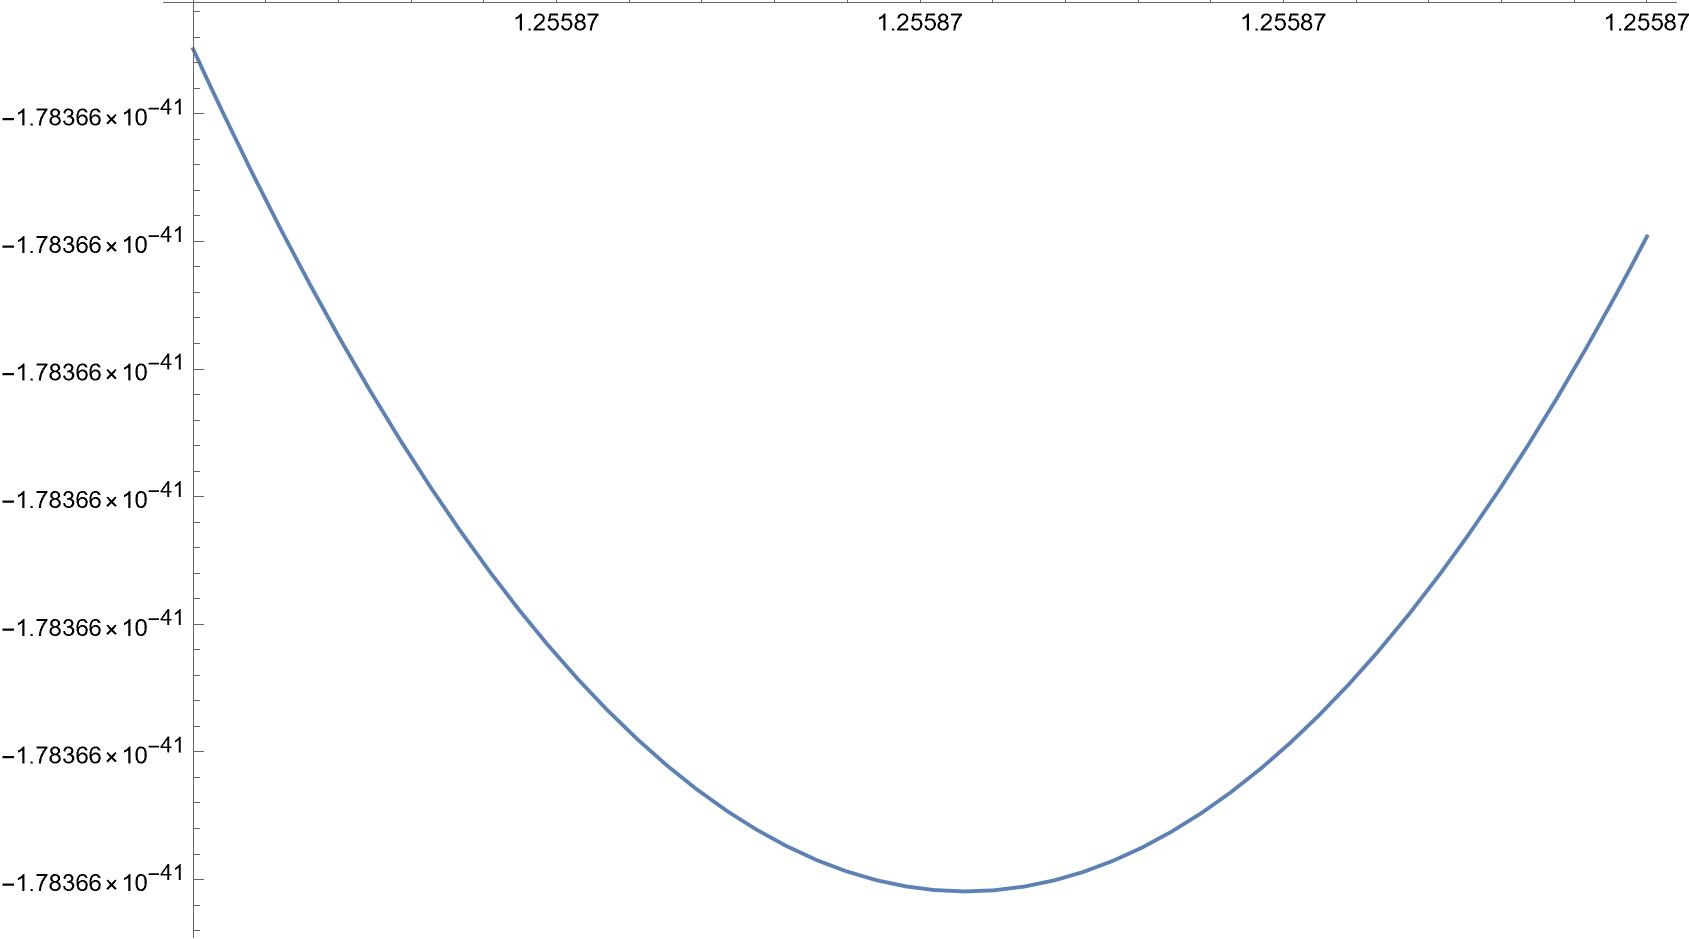
\includegraphics[width=0.8\textwidth]{fig/kklt_minimum.jpg}
   \caption{KKLT模型の$F$-termポテンシャル}
   \label{plot_KKLT_model}
\end{figure}

Polonyi-KKLT模型のスーパーポテンシャルとケーラーポテンシャルは
\begin{equation}
   \left\{
      \begin{alignedat}{1}
         W
         &=
         w_{0}
         -
         Ae^{-aT}
         +
         BX
         \\
         K
         &=
         -
         3\ln(T+\bar{T})
         +
         |X^2|
      \end{alignedat}
   \right.
   \nonumber
\end{equation}
である.このスーパーポテンシャルとケーラーポテンシャルによる$F$-termポテンシャルは図\ref{plot_Polonyi-KKLT_model}の通りである.ただし,パラメターは
\begin{equation}
   A=1
   ,\ 
   a=4 \pi^2
   ,\ 
   B=e^{-4\pi^2}
   ,\ 
   w_{0}
   \sim
   2.1659
   \times
   10^{-18}
   ,\ 
   X
   =
   \sqrt{3}-1
   \nonumber
\end{equation}
とした.この場合,最小点における値は
\begin{equation}
   \ev*{T}
   \sim
   1.085
   ,\ 
   \left.V\right|_{0}
   \sim
   6.1107\times 10^{-51}
   \label{minimum_Polonyi-KKLT}
\end{equation}
となる.2つの最小値の結果\eqref{minimum_KKLT},\ \eqref{minimum_Polonyi-KKLT}より,確かにポテンシャルの最小値がupliftされている\footnote{
   今回は,$w_{0}$のtuningを15桁まで行った.さらに現実的な真空を実現するためには,より高い精度でfine tuningすることが必要である.
}.

\begin{figure}[ht]
   \centering
   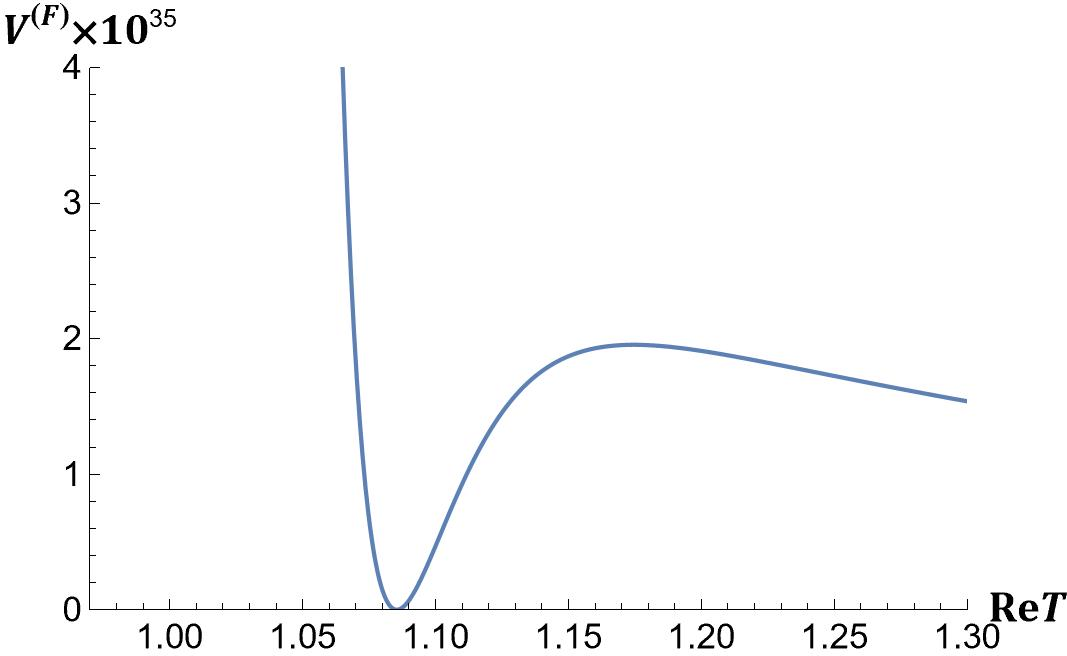
\includegraphics[width=0.8\textwidth]{fig/aaaa.jpg}
   \caption{Polonyi-KKLT模型の$F$-termポテンシャル}
   \label{plot_Polonyi-KKLT_model}
\end{figure}


\section{ケーラーモジュライの規格化}
\label{kahler_moduli_normalize}

(ケーラー)モジュライの運動項から,モジュライ場$T_{i}$の規格化を行う.モジュライの運動項は
\begin{equation}
   \mathcal{L}_{\text{kin}}
   =
   \sum_{r}
   K_{T_{r}T_{r}}
   \partial_{\mu}T_{r}
   \partial^{\mu}T^{r}
   \nonumber
\end{equation}
である.ここで,
\begin{equation}
   K
   =
   -
   \sum_{r}
   \ln(T_{r}+\bar{T}_{r})
   ,\quad
   K_{T_{r}T_{r}}
   =
   \frac{1}{(T_{r}+\bar{T}_{r})^2}
   \nonumber
\end{equation}
である.したがって,運動項の係数は,質量基底の変換$T_{r}=\sum P_{ri}\tilde{T}_{i}$によって
\begin{equation}
   \mathcal{L}_{\text{kin}}
   =
   \sum_{r}
   K_{T_{r}T_{r}}
   \partial_{\mu}T_{r}
   \partial^{\mu}T^{r}
   =
   \sum_{r}
   \frac{1}{\left(
      \displaystyle
      \sum_{i}P_{ri}\left(\ev*{\tilde{T}_{i}}+\ev*{\bar{\tilde{T}}_{i}}\right)\right)^2
   }   
   \partial_{\mu}\tilde{T}_{r}
   \partial^{\mu}\tilde{T}^{r}
   \nonumber
\end{equation}
となっている.したがって,モジュライを新しく
\begin{equation}
   T^{\prime}_{r}
   \equiv
   \dfrac{1}{\sum_{i}P_{ri}\left(\ev*{\tilde{T}_{i}}+\ev*{\bar{\tilde{T}}_{i}}\right)}\tilde{T}_{r}
   \nonumber
\end{equation}
と定義すれば
\begin{equation}
   \mathcal{L}
   =
   \sum_{r}\partial_{\mu}T^{\prime}_{r}\partial^{\mu}T^{\prime}_{r}
   \nonumber
\end{equation}
となる.このとき,モジュライ$T$の質量項は
\begin{equation}
   \sum_{r}\frac{1}{2}m_{r}\tilde{T}_{r}^2
   =
   \sum_{r}\frac{1}{2}
   \left\{
   \sum_{i}P_{ri}\left(\ev*{\tilde{T}_{i}}+\ev*{\bar{\tilde{T}}_{i}}\right)
   m_{r}
   \right\}
   {T^{\prime}_{r}}^2
   \nonumber
\end{equation}
となるため,質量は
\begin{equation}
   m_{r}^{\prime}
   =   
   \sum_{i}P_{ri}\left(\ev*{\tilde{T}_{i}}+\ev*{\bar{\tilde{T}}_{i}}\right)
   m_{r}
   \label{normalized_mass}
\end{equation}
と規格化される.


\section{作用\texorpdfstring{\eqref{action_4dSUGRA}}{2.9}における\texorpdfstring{$F$}{F}-termポテンシャルの導出}

$F$-termポテンシャルは,作用\eqref{action_4dSUGRA}のうち
\begin{equation}
   -3
   \int\dd^4\theta\theta\ 
   \bar{C}Ce^{-K/3}
   +
   \int\dd\theta^2 C^3 W
   +
   \int\dd\bar{\theta}^2 \bar{C}^3 \bar{W}
   \nonumber
\end{equation}
から導出できる.$C^3 W$の$\theta^2$の項は
\begin{equation}
   C^3 W
   \left.\right|_{\theta\theta}
   =
   C_{0}^3 W_{\theta\theta}
   +
   3C^{2}_{0}C_{\theta\theta}
   W_{0}
   \label{eqn_append3_1}
\end{equation}
である.ここで
\begin{equation}
   \Phi^{I}
   =
   \phi^{I}+\cdots+\theta\theta F^{I}
   \ ,\ 
   C
   =
   \phi^{C}+\cdots+\theta\theta F^{C}
   \nonumber
\end{equation}
とする.$\Phi^{I},C$はカイラル超場であるため,上式のように展開できる.スーパーポテンシャル$W$はカイラル超場$\Phi^{I}$の正則なポテンシャルであるため
\begin{equation}
   W[\Phi]
   =
   w_{0}+w_{1}\pdv{W}{\Phi^{I}}\Phi^{I}+\frac{w_{2}}{2}\pdv{W}{\Phi^{I}}{\Phi^{J}}\Phi^{I}\Phi^{J}+\cdots
   \nonumber
\end{equation}
であり,したがって
\begin{align}
   W_{\theta\theta}
   &=
   \Phi^{I}_{\theta\theta}w_{1}\pdv{W}{\Phi^{I}}
   +
   \Phi^{I}_{\theta\theta}w_{2}\pdv{W}{\Phi^{I}}{\Phi^{J}}\Phi^{J}+\cdots
   \nonumber
   \\
   &=
   F^{I}W_{I}
   \nonumber
\end{align}
である.よって,
\begin{equation}
   C^{3}W\left.\right|_{\theta\theta}
   =
   C_{0}^3W_{I}F^{I}
   +
   3C_{0}^{2}F^{C}W_{0}
   \label{eqn_append3_2}
\end{equation}
である.$\bar{C}^3 \bar{W}$についても同様にすれば
\begin{equation}
   \bar{C}^3 \bar{W}\left.\right|_{\theta\theta}
   =
   \bar{C}_{0}^{3}\bar{W}_{\bar{J}}\bar{F}^{\bar{J}}
   +
   3\bar{C}_{0}^{2}\bar{F}^{\bar{C}}\bar{W}_{0}
   \label{eqn_append3_3}
\end{equation}
である.同様にして,ケーラーポテンシャルによる寄与を計算すると
\begin{align}
   -3\bar{C}Ce^{-K/3}\left.\right|_{\theta\theta\overline{\theta\theta}}
   &=
   -3\bar{F}^{\bar{C}}F^{C}e^{-K/3}\left.\right|_{0}
   -
   3\bar{F}^{\bar{C}}C_{0}e^{-K/3}\left.\right|_{\theta\theta}
   \nonumber
   \\
   &\qquad
   -3\bar{C}_{0}F^{C}e^{-K/3}\left.\right|_{\overline{\theta\theta}}
   -
   3\bar{C}_{0}C_{0}e^{-K/3}\left.\right|_{\theta\theta\overline{\theta\theta}}
   \nonumber
   \\
   &=  
   -3\bar{F}^{C}F^{C}e^{-K_{0}/3}
   +
   \bar{F}^{C}C_{0}e^{-K_{0}/3}\partial_{I}K_{0}F^{I}
   \nonumber
   \\
   &\qquad
   +
   \bar{C}_{0}F^{C}e^{-K_{0}/3}\partial_{\bar{J}}K_{0}F^{\bar{J}}
   \nonumber
   \\
   &\qquad
   +
   e^{-K_{0}/3}|C_{0}|^2
   \left(
       \partial_{I\bar{J}}K_{0}F^{I}F^{\bar{J}}
       -
       \frac{1}{3}\partial_{I}K_{0}\partial_{\bar{J}}K_{0}F^{I}F^{\bar{J}}
   \right)
   \label{eqn_append3_4}
\end{align}
である.\eqref{eqn_append3_2},\eqref{eqn_append3_3},\eqref{eqn_append3_4}を\eqref{eqn_append3_1}に代入すると
\begin{align}
   &
   -
   3\bar{F}^{C}F^{C}e^{-K_{0}/3}
   +
   \bar{F}^{C}C_{0}e^{-K_{0}/3}\partial_{I}K_{0}F^{I}
   \nonumber
   \\
   &\qquad
   +
   \bar{C}_{0}F^{C}e^{-K_{0}/3}\partial_{\bar{J}}K_{0}F^{\bar{J}}
   \nonumber
   \\
   &\qquad
   +
   e^{-K_{0}/3}|C_{0}|^2
   \left(
       \partial_{I\bar{J}}K_{0}F^{I}F^{\bar{J}}
       -
       \frac{1}{3}\partial_{I}K_{0}\partial_{\bar{J}}K_{0}F^{I}F^{\bar{J}}
   \right)
   \nonumber
   \\
   &\qquad
   +
   C_{0}^3W_{I}F^{I}
   +
   3C_{0}^{2}F^{C}W_{0}
   \nonumber
   \\
   &\qquad
   +
   \bar{C}_{0}^{3}\bar{W}_{\bar{J}}\bar{F}^{\bar{J}}
   +
   3\bar{C}_{0}^{2}\bar{F}^{\bar{C}}\bar{W}_{0}
   \label{append3_F-term}
\end{align}
である.補助場$F^{C},\ \bar{F}^{\bar{C}}$についての運動方程式は
\begin{equation}
    \left\{ 
    \begin{alignedat}{1}
        F^{C}
        &=
        \frac{1}{3}C_{0}K_{I}F^{I}
        +
        \bar{C}_{0}^{2}\bar{W}_{0}e^{K_{0}/3}
        ,
        \\
        \bar{F}^{C}
        &=
        \frac{1}{3}\bar{C}_{0}K_{\bar{J}}F^{\bar{J}}
        +
        C_{0}^{2}W_{0}e^{K_{0}/3}
        .            
    \end{alignedat}
    \right.
    \nonumber
\end{equation}
となるので,\eqref{append3_F-term}に代入すれば
\begin{align}
   &
       -3
       \left(
           \frac{1}{3}C_{0}K_{I}F^{I}
           +
           \bar{C}_{0}^{2}\bar{W}_{0}e^{K_{0}/3}            
       \right)
       \left(
           \frac{1}{3}\bar{C}_{0}K_{\bar{J}}F^{\bar{J}}
           +
           C_{0}^{2}W_{0}e^{K_{0}/3}
       \right)
       e^{-K_{0}/3}
   \nonumber
   \\
   &\qquad
       +
       \left(
           \frac{1}{3}\bar{C}_{0}K_{\bar{J}}F^{\bar{J}}
           +
           C_{0}^{2}W_{0}e^{K_{0}/3}
       \right)
       C_{0}e^{-K_{0}/3}K_{I}F^{I}
   \nonumber
   \\
   &\qquad
       +
       \bar{C}_{0}
       \left(
           \frac{1}{3}C_{0}K_{I}F^{I}
           +
           \bar{C}_{0}^{2}\bar{W}_{0}e^{K_{0}/3}            
       \right)
       e^{-K_{0}/3}K_{\bar{J}}F^{\bar{J}}
   \nonumber
   \\
   &\qquad
       +
       e^{-K_{0}/3}|C_{0}|^2
       \left(
           K_{I\bar{J}}F^{I}F^{\bar{J}}
           -
           \frac{1}{3}K_{I}K_{\bar{J}}F^{I}F^{\bar{J}}
       \right)
   \nonumber   
   \\
   &\qquad
       +
       C_{0}^{3}W_{I}F^{I}
       +
       \bar{C}_{0}^{3}\bar{W}_{\bar{J}}F^{\bar{J}}
   \nonumber   
   \\
   &\qquad
       +
       3C_{0}^2
       \left(
           \frac{1}{3}C_{0}K_{I}F^{I}
           +
           \bar{C}_{0}^{2}\bar{W}_{0}e^{K_{0}/3}
       \right)
       W_{0}
   \nonumber   
   \\
   &\qquad
       +
       3\bar{C}_{0}^2
       \left(
           \frac{1}{3}\bar{C}_{0}K_{\bar{J}}F^{\bar{J}}
           +
           C_{0}^{2}W_{0}e^{K_{0}/3}
       \right)
       \bar{W}_{0}
   \nonumber
   \\
   &=
   C_{0}^{3}W_{0}K_{I}F^{I}
   +
   \bar{C}_{0}^{3}\bar{W}_{0}K_{\bar{J}}F^{\bar{J}}
   \nonumber
   \\
   &\qquad
   +
   e^{-K_{0}/3}
   |C_{0}|^2K_{I\bar{J}}F^{I}F^{\bar{J}}
   +
   3
   |C_{0}|^{4}|W_{0}|^{2}e^{K_{0}/3}
   \nonumber
   \\
   &\qquad
   +
   C_{0}^{3}W_{I}F^{I}
   +
   \bar{C}_{0}^3\bar{W}_{\bar{J}}F^{\bar{J}}
   \label{eqn_append3_5}
\end{align}
であるため,補助場$F^{I},\ \bar{F}^{\bar{J}}$の運動方程式
\begin{equation}
    \left\{
    \begin{alignedat}{1}
        F^{\bar{J}}
        &=
        \frac{C_{0}^{3}}{|C_{0}|^{2}}e^{K_{0}/3}K^{I\bar{J}}
        \left(
            -
            W_{0}K_{I}
            -
            W_{I}
        \right)
        ,
        \\
        F^{I}
        &=
        \frac{\bar{C}_{0}^{3}}{|C_{0}|^2}e^{K_{0}/3}K^{I\bar{J}}
        \left(
            -
            \bar{W}_{0}K_{\bar{J}}
            -
            W_{\bar{J}}
        \right)
        .            
    \end{alignedat}
    \right.
    \nonumber
\end{equation}
を代入すれば,\eqref{eqn_append3_5}は
\begin{align}
&
C_{0}^{3}
W_{0}K_{I}
\cdot
    \frac{\bar{C}_{0}^{3}}{|C_{0}|^2}e^{K_{0}/3}K^{I\bar{J}}
    \left(
        -
        \bar{W}_{0}K_{\bar{J}}
        -
        W_{\bar{J}}
    \right)
\nonumber
\\
&\quad
+\bar{C}_{0}^{3}\bar{W}_{0}K_{\bar{J}}
\cdot
    \frac{C_{0}^{3}}{|C_{0}|^{2}}e^{K_{0}/3}K^{I\bar{J}}
    \left(
        -
        W_{0}K_{I}
        -
        W_{I}
    \right)
\nonumber
\\
&\quad
+
e^{K_{0}/3}|C_{0}|^{4}K_{I\bar{J}}K^{I\bar{J^{\prime}}}K^{I^{\prime}\bar{J}}
    \left(
        -
        \bar{W}_{0}K_{\bar{J^{\prime}}}
        -
        W_{\bar{J^{\prime}}}
    \right)
    \left(
        -
        W_{0}K_{I^{\prime}}
        -
        W_{I^{\prime}}
    \right)
\nonumber   
\\
&\quad
+
3
e^{K_{0}}|C_{0}|^{4}|W_{0}|^2
\nonumber   
\\
&\quad
+
C_{0}^{3}W_{I}
\cdot
    \frac{\bar{C}_{0}^{3}}{|C_{0}|^2}e^{K_{0}/3}K^{I\bar{J}}
    \left(
        -
        \bar{W}_{0}K_{\bar{J}}
        -
        W_{\bar{J}}
    \right)
\nonumber
\\
&\quad
+
\bar{C}^{0}W_{\bar{J}}
\cdot
    \frac{C_{0}^{3}}{|C_{0}|^{2}}e^{K_{0}/3}K^{I\bar{J}}
    \left(
        -
        W_{0}K_{I}
        -
        W_{I}
    \right)
\nonumber   
\\
&=
-
e^{K_{0}/3}|C_{0}|^{4}\left[\vphantom{\dfrac{1}{2}}\right.
    K^{I\bar{J}}W_{I}W_{\bar{J}}
    +
    K^{I\bar{J}}W_{I}K_{\bar{J}}\bar{W}_{0}
\nonumber
\\
&\qquad
+
K^{I\bar{J}}K_{I}W_{\bar{J}}W_{0}
+
K^{I\bar{J}}K_{I}K_{\bar{J}}|W_{0}|^2
-
3|W_{0}|^2
\left.\vphantom{\dfrac{1}{2}}\right]
\nonumber
\\
&\equiv
-
e^{K}
\left(
    K^{I\bar{J}}
    (D_{I}W)(D_{\bar{J}}\bar{W})
    -
    3|W|^2
\right)    
\nonumber   
\end{align}
である.ただし,
\begin{equation}
   D_{I}W_{0}
   \equiv
   W_{I}
   +
   K_{I}W_{0}
   \nonumber
\end{equation}
とし,
\begin{equation}
   C_{0}
   =
   \bar{C}_{0}
   =
   e^{K_{0}/6}
   \nonumber
\end{equation}
とゲージ固定した.また,$K_{0}\equiv K,\ W_{0}\equiv W$とした.したがって,$F$-termポテンシャルは
\begin{equation}
   V^{(F)}
   =
   e^{K}
   \left(
       K^{I\bar{J}}
       (D_{I}W)(D_{\bar{J}}\bar{W})
       -
       3|W|^2
   \right)    
\end{equation}
である.


\clearpage
\bibliography{hoge}
\bibliographystyle{ytphys}

\nocite{柴崎_背景_2021}
\nocite{中野_磁化_2023}

\end{document}
